\chapter{Exercicis proposats}
\label{cap:exercicis-proposats}

\section{Construcció i representació dels nombres racionals}

\begin{exercici}[Fraccions equivalents]
	Decideix quines de les fraccions següents representen el mateix nombre racional:
	\[
	\frac{8}{12},
	\qquad
	\frac{10}{15},
	\qquad
	\frac{-4}{-6},
	\qquad
	\frac{14}{18}.
	\]
\end{exercici}

\begin{indicacio}
	Recorda que dues fraccions \(a/b\) i \(c/d\), amb \(b,d\neq0\), representen el mateix nombre racional si i només si \(ad=bc\). També pots reduir totes les fraccions a forma irreductible.
\end{indicacio}

\begin{exercici}[Classe d'equivalència]
	Escriu cinc representants diferents del nombre racional representat per
	\[
	\frac{5}{-8}.
	\]
\end{exercici}

\begin{indicacio}
	Primer escriu la fracció amb denominador positiu. Després multiplica numerador i denominador pel mateix enter no nul.
\end{indicacio}

\begin{exercici}[Els enters com a racionals]
	Escriu els nombres enters següents com a nombres racionals i dona tres representants fraccionaris diferents de cadascun:
	\[
	-4,
	\qquad
	0,
	\qquad
	7.
	\]
\end{exercici}

\begin{indicacio}
	Recorda que un enter \(n\) s'identifica amb el racional \(\left[\frac{n}{1}\right]\). Multiplica numerador i denominador pel mateix enter no nul per obtenir representants diferents.
\end{indicacio}

\begin{exercici}[Fracció irreductible]
	Redueix a forma irreductible les fraccions següents:
	\[
	\frac{72}{120},
	\qquad
	\frac{-135}{180},
	\qquad
	\frac{154}{-210}.
	\]
\end{exercici}

\begin{indicacio}
	Calcula el màxim comú divisor del numerador i del denominador en cada cas. Escriu sempre el resultat final amb denominador positiu.
\end{indicacio}

\begin{exercici}[Signe d'un racional]
	Escriu les fraccions següents en forma irreductible i amb denominador positiu:
	\[
	\frac{-18}{-42},
	\qquad
	\frac{25}{-35},
	\qquad
	\frac{-44}{66}.
	\]
\end{exercici}

\begin{indicacio}
	Recorda que dos signes negatius es cancel·len. Si només hi ha un signe negatiu, el nombre racional és negatiu.
\end{indicacio}

\begin{exercici}[Representació amb el teorema de Tales]
	Construeix sobre la recta numèrica, mitjançant el teorema de Tales, els punts corresponents a
	\[
	\frac{3}{5}
	\qquad\text{i}\qquad
	-\frac{4}{7}.
	\]
\end{exercici}

\begin{indicacio}
	Per situar \(\frac{3}{5}\), divideix el segment \([0,1]\) en cinc parts iguals amb una semirecta auxiliar. Per situar \(-\frac{4}{7}\), divideix el segment \([0,-1]\) en set parts iguals.
\end{indicacio}

\begin{exercici}[Racionals majors que la unitat]
	Construeix sobre la recta numèrica, amb el teorema de Tales, els punts corresponents a
	\[
	\frac{7}{3}
	\qquad\text{i}\qquad
	-\frac{9}{4}.
	\]
\end{exercici}

\begin{indicacio}
	Usa la divisió euclidiana:
	\[
	7=3\cdot2+1,
	\qquad
	9=4\cdot2+1.
	\]
	Així, \(\frac{7}{3}=2+\frac{1}{3}\) i \(-\frac{9}{4}=-2-\frac{1}{4}\).
\end{indicacio}

\section{Operacions amb nombres racionals}

\begin{exercici}[Addició i subtracció]
	Calcula i simplifica:
	\[
	\frac{5}{6}
	-
	\frac{7}{9}
	+
	\frac{1}{12}.
	\]
\end{exercici}

\begin{indicacio}
	Busca el mínim comú múltiple dels denominadors \(6\), \(9\) i \(12\), expressa totes les fraccions amb aquest denominador i opera els numeradors.
\end{indicacio}

\begin{exercici}[Multiplicació de fraccions]
	Calcula i simplifica:
	\[
	\frac{-14}{15}\cdot\frac{25}{21}.
	\]
\end{exercici}

\begin{indicacio}
	Abans de multiplicar, mira si pots simplificar factors del numerador amb factors del denominador.
\end{indicacio}

\begin{exercici}[Divisió de racionals]
	Calcula:
	\[
	\frac{-9}{14}:\frac{27}{35}.
	\]
\end{exercici}

\begin{indicacio}
	Dividir per un racional no nul és multiplicar pel seu invers. Transforma la divisió en una multiplicació i simplifica.
\end{indicacio}

\begin{exercici}[Oposat i invers]
	Troba l'oposat i l'invers dels nombres racionals següents:
	\[
	-\frac{6}{11},
	\qquad
	\frac{13}{-7},
	\qquad
	\frac{9}{4}.
	\]
\end{exercici}

\begin{indicacio}
	L'oposat canvia el signe del nombre. L'invers d'una fracció no nul·la s'obté intercanviant numerador i denominador.
\end{indicacio}

\begin{exercici}[Operació amb inversos]
	Calcula:
	\[
	\left(\frac{5}{8}\right)^{-1}
	+
	\left(-\frac{3}{4}\right)^{-1}.
	\]
\end{exercici}

\begin{indicacio}
	Calcula primer cada invers. Després fes l'addició amb denominador comú.
\end{indicacio}

\section{Ordre, densitat i valor absolut}

\begin{exercici}[Ordre en \(\Q\)]
	Ordena de menor a major:
	\[
	-\frac{2}{3},
	\qquad
	-\frac{5}{8},
	\qquad
	\frac{3}{10},
	\qquad
	\frac{4}{7}.
	\]
\end{exercici}

\begin{indicacio}
	Separa primer els nombres negatius dels positius. Per comparar fraccions positives, pots usar productes creuats o expressar-les amb denominador comú.
\end{indicacio}

\begin{exercici}[Comparació de racionals]
	Determina si són certes o falses les desigualtats següents:
	\[
	\frac{7}{12}<\frac{5}{8},
	\qquad
	-\frac{4}{9}<-\frac{3}{7},
	\qquad
	\frac{-6}{15}>\frac{-3}{5}.
	\]
\end{exercici}

\begin{indicacio}
	En les fraccions positives pots comparar en creu. En les fraccions negatives, recorda que el nombre amb més valor absolut és el més petit.
\end{indicacio}

\begin{exercici}[Densitat dels racionals]
	Troba quatre nombres racionals diferents entre
	\[
	\frac{2}{5}
	\qquad\text{i}\qquad
	\frac{3}{5}.
	\]
\end{exercici}

\begin{indicacio}
	Escriu les dues fraccions amb un denominador comú més gran. Per exemple, pots multiplicar els denominadors per \(10\) o per \(20\) per obtenir més numeradors intermedis.
\end{indicacio}

\begin{exercici}[Mitjana de dos racionals]
	Comprova que
	\[
	\frac{\frac{1}{4}+\frac{2}{3}}{2}
	\]
	és un nombre racional situat entre \(\frac{1}{4}\) i \(\frac{2}{3}\).
\end{exercici}

\begin{indicacio}
	Calcula primer l'addició \(\frac{1}{4}+\frac{2}{3}\), després divideix per \(2\). Finalment compara el resultat amb els dos nombres inicials.
\end{indicacio}

\begin{exercici}[Valor absolut]
	Calcula:
	\[
	\left|-\frac{7}{5}\right|,
	\qquad
	\left|\frac{3}{8}-\frac{5}{6}\right|,
	\qquad
	\left|-\frac{4}{9}+\frac{1}{3}\right|.
	\]
\end{exercici}

\begin{indicacio}
	Calcula primer el nombre que hi ha dins del valor absolut. Després escriu-ne la distància a \(0\).
\end{indicacio}

\section{Expressions decimals, potències i arrels}

\begin{exercici}[Decimals finits]
	Decideix quines de les fraccions següents tenen expressió decimal finita:
	\[
	\frac{7}{20},
	\qquad
	\frac{11}{24},
	\qquad
	\frac{9}{40},
	\qquad
	\frac{5}{18}.
	\]
\end{exercici}

\begin{indicacio}
	Redueix cada fracció a forma irreductible. Una fracció irreductible té expressió decimal finita si el seu denominador només té factors primers \(2\) i \(5\).
\end{indicacio}

\begin{exercici}[Fracció generatriu d'un decimal finit]
	Calcula la fracció generatriu de
	\[
	4{,}375.
	\]
\end{exercici}

\begin{indicacio}
	Escriu el decimal com una fracció amb denominador una potència de \(10\). Després simplifica.
\end{indicacio}

\begin{exercici}[Decimal periòdic pur]
	Calcula la fracció generatriu de
	\[
	0{,}\overline{27}.
	\]
\end{exercici}

\begin{indicacio}
	Anomena \(x=0{,}\overline{27}\). Multiplica per \(100\) i resta l'equació inicial per eliminar el període.
\end{indicacio}

\begin{exercici}[Decimal periòdic mixt]
	Calcula la fracció generatriu de
	\[
	3{,}4\overline{18}.
	\]
\end{exercici}

\begin{indicacio}
	Anomena \(x=3{,}4\overline{18}\). Com que hi ha una xifra no periòdica i dues xifres periòdiques, compara \(10x\) i \(1000x\).
\end{indicacio}

\begin{exercici}[Potències]
	Calcula:
	\[
	\left(-\frac{3}{5}\right)^2,
	\qquad
	\left(-\frac{3}{5}\right)^3,
	\qquad
	\left(\frac{2}{7}\right)^4.
	\]
\end{exercici}

\begin{indicacio}
	Eleva numerador i denominador a l'exponent corresponent. Recorda que una potència d'exponent parell d'un nombre negatiu és positiva, mentre que una potència d'exponent senar és negativa.
\end{indicacio}

\begin{exercici}[Propietats de les potències]
	Simplifica, sempre que sigui possible:
	\[
	\left(\frac{2}{3}\right)^4\cdot\left(\frac{2}{3}\right)^2,
	\qquad
	\frac{\left(-\frac{5}{7}\right)^6}{\left(-\frac{5}{7}\right)^2},
	\qquad
	\left[\left(\frac{3}{4}\right)^2\right]^3.
	\]
\end{exercici}

\begin{indicacio}
	Usa les propietats de les potències de la mateixa base i la potència d'una potència.
\end{indicacio}

\begin{exercici}[Arrels]
	Decideix quins dels nombres següents són racionals:
	\[
	\sqrt{\frac{25}{36}},
	\qquad
	\sqrt{\frac{3}{16}},
	\qquad
	\sqrt{\frac{121}{49}},
	\qquad
	\sqrt[3]{-\frac{64}{125}}.
	\]
\end{exercici}

\begin{indicacio}
	Una arrel quadrada d'una fracció és racional quan tant el numerador com el denominador són quadrats perfectes, després d'haver escrit la fracció en forma irreductible. En les arrels cúbiques, fixa't si numerador i denominador són cubs perfectes.
\end{indicacio}

\section{Operacions combinades amb fraccions, potències i arrels}

\begin{exercici}[Prioritat de les operacions]
	Calcula i simplifica:
	\[
	\frac{3}{5}
	-
	\frac{7}{10}\cdot\frac{2}{3}
	+
	\frac{1}{4}:\frac{5}{8}.
	\]
\end{exercici}

\begin{indicacio}
	Primer fes la multiplicació i la divisió. Després resol les addicions i subtraccions.
\end{indicacio}

\begin{exercici}[Parèntesis i divisió]
	Calcula i simplifica:
	\[
	\left(\frac{5}{6}-\frac{1}{3}\right):\frac{2}{9}-\frac{3}{4}.
	\]
\end{exercici}

\begin{indicacio}
	Primer resol el parèntesi. Després transforma la divisió en una multiplicació per l'invers.
\end{indicacio}

\begin{exercici}[Potències i parèntesis]
	Calcula:
	\[
	\left(-\frac{2}{3}\right)^2
	-
	\frac{5}{6}\left(\frac{3}{5}-\frac{1}{10}\right).
	\]
\end{exercici}

\begin{indicacio}
	Primer calcula la potència i el parèntesi. Després fes la multiplicació i, finalment, la subtracció.
\end{indicacio}

\begin{exercici}[Potències, arrels i signes]
	Calcula:
	\[
	\sqrt{\frac{25}{36}}
	+
	\sqrt[3]{-\frac{8}{27}}
	-
	\left(-\frac{1}{2}\right)^3.
	\]
\end{exercici}

\begin{indicacio}
	Calcula cada terme per separat. Recorda que l'arrel quadrada principal és no negativa i que les arrels cúbiques poden ser negatives.
\end{indicacio}

\begin{exercici}[Operació combinada completa]
	Calcula i simplifica:
	\[
	\left(\frac{2}{3}-\frac{5}{4}\right)^2
	+
	\sqrt{\frac{49}{81}}
	-
	\frac{3}{5}:\left(-\frac{9}{10}\right).
	\]
\end{exercici}

\begin{indicacio}
	Resol primer el parèntesi, la potència i l'arrel. Després transforma la divisió en una multiplicació per l'invers.
\end{indicacio}

\section{Raons, proporcions i proporcionalitat aritmètica}

\begin{exercici}[Raons]
	En una classe hi ha \(18\) alumnes que fan esport regularment i \(12\) alumnes que no en fan. Calcula:
	\begin{enumerate}[label=\alph*)]
		\item la raó entre alumnes que fan esport i alumnes que no en fan;
		\item la raó entre alumnes que fan esport i el total d'alumnes;
		\item la raó entre alumnes que no fan esport i el total d'alumnes.
	\end{enumerate}
\end{exercici}

\begin{indicacio}
	Una raó és un quocient entre dues quantitats. Abans de calcular les raons amb el total, calcula quants alumnes hi ha en total.
\end{indicacio}

\begin{exercici}[Proporcions]
	Determina si les igualtats següents són proporcions:
	\[
	\frac{6}{10}=\frac{9}{15},
	\qquad
	\frac{8}{14}=\frac{12}{21},
	\qquad
	\frac{5}{9}=\frac{20}{36}.
	\]
\end{exercici}

\begin{indicacio}
	Comprova si el producte dels mitjans és igual al producte dels extrems.
\end{indicacio}

\begin{exercici}[Propietats de les proporcions]
	A partir de la proporció
	\[
	\frac{12}{18}=\frac{20}{30},
	\]
	escriu tres proporcions equivalents usant propietats de les proporcions.
\end{exercici}

\begin{indicacio}
	Pots usar la inversió dels termes, l'alternança dels termes o la propietat de sumar els termes de cada raó.
\end{indicacio}

\begin{exercici}[Tercera proporcional]
	Troba la tercera proporcional de \(4\) i \(10\).
\end{exercici}

\begin{indicacio}
	Busca \(x\) tal que
	\[
	\frac{4}{10}=\frac{10}{x}.
	\]
\end{indicacio}

\begin{exercici}[Quarta proporcional]
	Troba la quarta proporcional de \(6\), \(15\) i \(14\).
\end{exercici}

\begin{indicacio}
	Busca \(x\) tal que
	\[
	\frac{6}{15}=\frac{14}{x}.
	\]
\end{indicacio}

\begin{exercici}[Mitjana proporcional]
	Determina si existeix en \(\Q\) la mitjana proporcional positiva de les parelles següents:
	\[
	4\text{ i }25,
	\qquad
	2\text{ i }8,
	\qquad
	3\text{ i }12.
	\]
\end{exercici}

\begin{indicacio}
	Si \(x\) és la mitjana proporcional positiva de \(a\) i \(b\), aleshores \(x^2=ab\). Mira si \(ab\) és un quadrat d'un nombre racional.
\end{indicacio}

\begin{exercici}[Relació entre magnituds]
	Observa la taula següent:
	\[
	\begin{array}{c|cccc}
	x & 2 & 4 & 6 & 8 \\
	\hline
	y & 5 & 10 & 15 & 20
	\end{array}
	\]
	Determina si les magnituds són directament proporcionals, inversament proporcionals o cap de les dues coses.
\end{exercici}

\begin{indicacio}
	No miris només si les dues magnituds augmenten. Comprova si el quocient \(y/x\) és constant o si el producte \(xy\) és constant.
\end{indicacio}

\begin{exercici}[Relació entre magnituds]
	Observa la taula següent:
	\[
	\begin{array}{c|cccc}
	x & 3 & 4 & 6 & 12 \\
	\hline
	y & 16 & 12 & 8 & 4
	\end{array}
	\]
	Determina si les magnituds són directament proporcionals, inversament proporcionals o cap de les dues coses.
\end{exercici}

\begin{indicacio}
	Calcula els productes \(xy\) i els quocients \(y/x\). Decideix quina relació es manté constant.
\end{indicacio}

\begin{exercici}[Relació entre magnituds]
	En una taula de valors es té:
	\[
	\begin{array}{c|cccc}
	x & 1 & 2 & 3 & 4 \\
	\hline
	y & 3 & 7 & 11 & 15
	\end{array}
	\]
	Determina si hi ha proporcionalitat directa, proporcionalitat inversa o cap de les dues.
\end{exercici}

\begin{indicacio}
	Que una magnitud augmenti quan l'altra augmenta no garanteix que hi hagi proporcionalitat directa. Comprova si \(y/x\) és constant.
\end{indicacio}

\section{Aplicacions a problemes de la vida real}

\begin{exercici}[Recepta]
	Una recepta per a \(4\) persones necessita \(300\) g d'arròs i \(120\) g de verdures. Vols preparar-la per a \(10\) persones.
	\begin{enumerate}[label=\alph*)]
		\item Quina relació hi ha entre el nombre de persones i la quantitat d'arròs?
		\item Quants grams d'arròs calen?
		\item Quants grams de verdures calen?
	\end{enumerate}
\end{exercici}

\begin{indicacio}
	Primer decideix si, en augmentar el nombre de persones, les quantitats d'ingredients augmenten en la mateixa proporció.
\end{indicacio}

\begin{exercici}[Feina compartida]
	Tres persones, treballant al mateix ritme, acaben una feina en \(8\) hores. Quantes hores trigaran sis persones a fer la mateixa feina, si totes treballen al mateix ritme?
\end{exercici}

\begin{indicacio}
	Abans de calcular, decideix si en augmentar el nombre de persones el temps augmenta o disminueix. Mira quin producte es manté constant.
\end{indicacio}

\begin{exercici}[Producció]
	Una màquina fabrica \(450\) peces en \(3\) hores. Una altra màquina igual treballa durant \(7\) hores.
	\begin{enumerate}[label=\alph*)]
		\item Quantes peces fabricarà?
		\item Quantes hores caldrien per fabricar \(1200\) peces?
	\end{enumerate}
\end{exercici}

\begin{indicacio}
	Si el ritme de producció es manté constant, el nombre de peces i el temps són magnituds directament proporcionals.
\end{indicacio}

\begin{exercici}[Comparació de preus]
	En una botiga, un paquet de \(6\) iogurts costa \(2{,}70\) euros. En una altra botiga, un paquet de \(10\) iogurts costa \(4{,}30\) euros. Quin paquet és més econòmic per iogurt?
\end{exercici}

\begin{indicacio}
	Calcula el preu d'un iogurt en cada cas. Estàs comparant dues raons.
\end{indicacio}

\begin{exercici}[Mescla]
	Per preparar una beguda isotònica es barregen \(3\) parts d'aigua amb \(1\) part de concentrat. Si vols preparar \(2\) litres de beguda, quina quantitat d'aigua i de concentrat necessites?
\end{exercici}

\begin{indicacio}
	En total hi ha \(4\) parts. Expressa quina fracció del total correspon a l'aigua i quina fracció correspon al concentrat.
\end{indicacio}

\begin{exercici}[Percentatge de descompte]
	Un llibre costa \(32\) euros i té un descompte del \(25\%\). Quin és el preu final?
\end{exercici}

\begin{indicacio}
	Calcula primer el \(25\%\) de \(32\). Després resta aquest descompte al preu inicial.
\end{indicacio}

\begin{exercici}[Percentatge d'augment]
	El preu d'un servei era de \(80\) euros i augmenta un \(12\%\). Quin és el nou preu?
\end{exercici}

\begin{indicacio}
	Calcula el \(12\%\) de \(80\) i suma aquest increment al preu inicial.
\end{indicacio}

\begin{exercici}[Velocitat i temps]
	Un trajecte de \(180\) km es fa a una velocitat mitjana constant. Si es circula a \(90\) km/h, es triga \(2\) hores. Quant es trigarà si es circula a \(120\) km/h?
\end{exercici}

\begin{indicacio}
	La distància és fixa. Decideix si la velocitat i el temps són directament o inversament proporcionals.
\end{indicacio}

\begin{exercici}[Repartiment segons aportacions]
	Tres persones han invertit \(200\), \(300\) i \(500\) euros en un projecte. Al final obtenen un benefici de \(1200\) euros, que es reparteix segons l'aportació inicial de cadascú. Quant rep cada persona?
\end{exercici}

\begin{indicacio}
	El benefici s'ha de repartir en la mateixa proporció que les aportacions. Calcula primer la suma total invertida.
\end{indicacio}

\begin{exercici}[Repartiment segons eficiència]
	Tres equips han de repartir-se una gratificació de \(900\) euros. L'equip A ha trigat \(6\) hores a fer una mateixa tasca, l'equip B \(4\) hores i l'equip C \(3\) hores. La gratificació es reparteix segons la rapidesa demostrada. Quant correspon a cada equip?
\end{exercici}

\begin{indicacio}
	Si es premia la rapidesa, qui triga menys ha de rebre més. Reparteix de manera directament proporcional als inversos dels temps.
\end{indicacio}

\begin{exercici}[Problema amb decisió prèvia]
	En una excursió, el cost total d'un autobús és de \(540\) euros. Si hi van \(30\) alumnes, cada alumne paga \(18\) euros. Quant pagarà cada alumne si finalment hi van \(45\) alumnes?
\end{exercici}

\begin{indicacio}
	El cost total és fix. Decideix què passa amb el preu per alumne quan augmenta el nombre d'alumnes.
\end{indicacio}

\section{Proporcionalitat geomètrica i funcions de proporcionalitat}

\begin{exercici}[Escales]
	En un mapa a escala \(1:50000\), la distància entre dos pobles és de \(7{,}5\) cm. Quina és la distància real en quilòmetres?
\end{exercici}

\begin{indicacio}
	L'escala \(1:50000\) vol dir que \(1\) cm en el mapa representa \(50000\) cm en la realitat. Converteix després els centímetres reals en metres i quilòmetres.
\end{indicacio}

\begin{exercici}[Maquetes]
	Una maqueta està feta a escala \(1:75\). Si una paret real fa \(9\) m, quina longitud tindrà en la maqueta?
\end{exercici}

\begin{indicacio}
	Expressa primer \(9\) m en centímetres. Després divideix per \(75\), perquè la maqueta és \(75\) vegades més petita que la realitat.
\end{indicacio}

\begin{exercici}[Figures semblants]
	Dos triangles semblants tenen costats corresponents de longituds \(8\) cm i \(12\) cm. Si un altre costat del primer triangle fa \(14\) cm, quant fa el costat corresponent del segon triangle?
\end{exercici}

\begin{indicacio}
	Calcula primer el factor d'escala
	\[
	k=\frac{12}{8}.
	\]
	Després multiplica el costat de \(14\) cm per aquest factor.
\end{indicacio}

\begin{exercici}[Teorema de Tales]
	Dues rectes secants són tallades per rectes paral·leles. En una secant apareixen dos segments de \(5\) cm i \(8\) cm. En l'altra secant, el segment corresponent al de \(5\) cm fa \(15\) cm. Quant fa el segment corresponent al de \(8\) cm?
\end{exercici}

\begin{indicacio}
	Aplica el teorema de Tales. Si \(x\) és el segment desconegut, pots plantejar una proporció del tipus
	\[
	\frac{5}{8}=\frac{15}{x}.
	\]
\end{indicacio}

\begin{exercici}[Funció associada a una relació de proporcionalitat]
	Un quilogram de farina costa \(1{,}60\) euros.
	\begin{enumerate}[label=\alph*)]
		\item Escriu la funció que dona el preu total \(y\) en funció dels quilograms comprats \(x\).
		\item Calcula el preu de \(2{,}5\) kg.
		\item Completa una taula per a \(x=0\), \(1\), \(2\), \(3\) i \(4\).
	\end{enumerate}
\end{exercici}

\begin{indicacio}
	El preu total és proporcional a la quantitat comprada. La funció és de la forma \(y=kx\).
\end{indicacio}

\begin{exercici}[Representació de punts d'una funció directa]
	Considera la funció
	\[
	f(x)=\frac{3}{2}x.
	\]
	Calcula \(f(x)\) per a
	\[
	x=-2,
	\quad
	x=-1,
	\quad
	x=0,
	\quad
	x=1,
	\quad
	x=2,
	\]
	i representa només els punts obtinguts, sense traçar una línia contínua.

	\begin{center}
	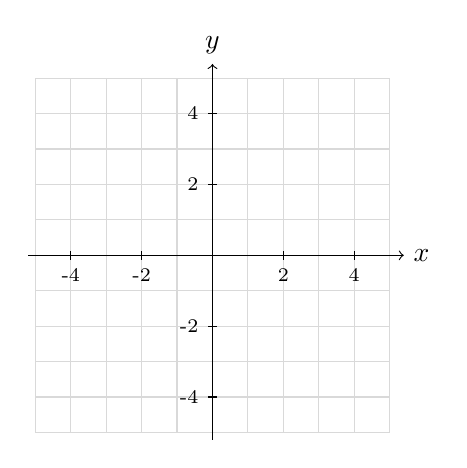
\begin{tikzpicture}[scale=0.45]
		\draw[step=1,gray!30,thin] (-5,-5) grid (5,5);
		\draw[->] (-5.2,0) -- (5.4,0) node[right] {$x$};
		\draw[->] (0,-5.2) -- (0,5.4) node[above] {$y$};
		\foreach \x in {-4,-2,2,4} {
			\draw (\x,0.12) -- (\x,-0.12) node[below] {\scriptsize \x};
		}
		\foreach \y in {-4,-2,2,4} {
			\draw (0.12,\y) -- (-0.12,\y) node[left] {\scriptsize \y};
		}
	\end{tikzpicture}
	\end{center}
\end{exercici}

\begin{indicacio}
	Substitueix cada valor de \(x\) en la funció. Els punts obtinguts tenen coordenades \((x,f(x))\).
\end{indicacio}

\begin{exercici}[Funció associada a una relació inversa]
	Una feina requereix \(72\) hores de treball total. Si hi treballen \(x\) persones al mateix ritme, sigui \(y\) el temps necessari.
	\begin{enumerate}[label=\alph*)]
		\item Escriu la funció que dona \(y\) en funció de \(x\).
		\item Calcula el temps necessari si hi treballen \(8\) persones.
		\item Explica per què \(x=0\) no és un valor admissible.
	\end{enumerate}
\end{exercici}

\begin{indicacio}
	El producte entre el nombre de persones i el temps total es manté constant.
\end{indicacio}

\begin{exercici}[Representació de punts d'una funció inversa]
	Considera la funció
	\[
	f(x)=\frac{6}{x}.
	\]
	Calcula \(f(x)\) per a
	\[
	x=-6,
	\quad
	x=-3,
	\quad
	x=-2,
	\quad
	x=-1,
	\quad
	x=1,
	\quad
	x=2,
	\quad
	x=3,
	\quad
	x=6,
	\]
	i representa només els punts obtinguts, sense traçar una corba contínua.

	\begin{center}
	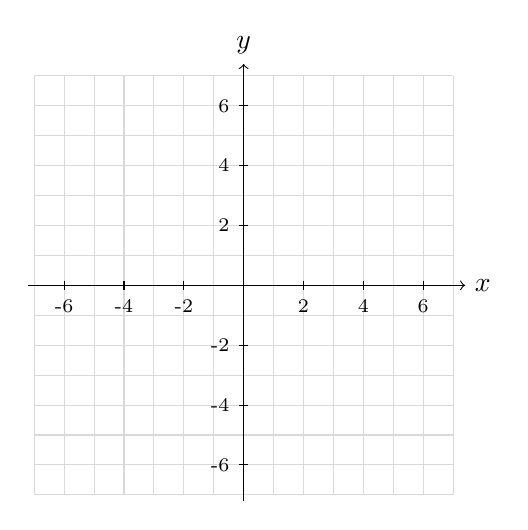
\begin{tikzpicture}[scale=0.38]
		\draw[step=1,gray!30,thin] (-7,-7) grid (7,7);
		\draw[->] (-7.2,0) -- (7.4,0) node[right] {$x$};
		\draw[->] (0,-7.2) -- (0,7.4) node[above] {$y$};
		\foreach \x in {-6,-4,-2,2,4,6} {
			\draw (\x,0.15) -- (\x,-0.15) node[below] {\scriptsize \x};
		}
		\foreach \y in {-6,-4,-2,2,4,6} {
			\draw (0.15,\y) -- (-0.15,\y) node[left] {\scriptsize \y};
		}
	\end{tikzpicture}
	\end{center}
\end{exercici}

\begin{indicacio}
	Substitueix cada valor de \(x\). Recorda que \(x=0\) no forma part del domini d'aquesta funció.
\end{indicacio}
